%%%%%%%%%%%%%%%%%%%%%%%%%%%%%%%%%%%%%%%%%
% Beamer Presentation
% LaTeX Template
% Version 1.0 (10/11/12)
%
% This template has been downloaded from:
% http://www.LaTeXTemplates.com
%
% License:
% CC BY-NC-SA 3.0 (http://creativecommons.org/licenses/by-nc-sa/3.0/)
%
%%%%%%%%%%%%%%%%%%%%%%%%%%%%%%%%%%%%%%%%%

%----------------------------------------------------------------------------------------
%	PACKAGES AND THEMES
%----------------------------------------------------------------------------------------

\documentclass{beamer}

\mode<presentation> {

% The Beamer class comes with a number of default slide themes
% which change the colors and layouts of slides. Below this is a list
% of all the themes, uncomment each in turn to see what they look like.

%\usetheme{default}
%\usetheme{AnnArbor}
%\usetheme{Antibes}
%\usetheme{Bergen}
%\usetheme{Berkeley}
%\usetheme{Berlin}
%\usetheme{Boadilla}
%\usetheme{CambridgeUS}
%\usetheme{Copenhagen}
%\usetheme{Darmstadt}
%\usetheme{Dresden}
%\usetheme{Frankfurt}
%\usetheme{Goettingen}
%\usetheme{Hannover}
%\usetheme{Ilmenau}
%\usetheme{JuanLesPins}
%\usetheme{Luebeck}
\usetheme{Madrid}
%\usetheme{Malmoe}
%\usetheme{Marburg}
%\usetheme{Montpellier}
%\usetheme{PaloAlto}
%\usetheme{Pittsburgh}
%\usetheme{Rochester}
%\usetheme{Singapore}
%\usetheme{Szeged}
%\usetheme{Warsaw}

% As well as themes, the Beamer class has a number of color themes
% for any slide theme. Uncomment each of these in turn to see how it
% changes the colors of your current slide theme.

%\usecolortheme{albatross}
%\usecolortheme{beaver}
%\usecolortheme{beetle}
%\usecolortheme{crane}
%\usecolortheme{dolphin}
%\usecolortheme{dove}
%\usecolortheme{fly}
%\usecolortheme{lily}
%\usecolortheme{orchid}
%\usecolortheme{rose}
%\usecolortheme{seagull}
%\usecolortheme{seahorse}
%\usecolortheme{whale}
%\usecolortheme{wolverine}

%\setbeamertemplate{footline} % To remove the footer line in all slides uncomment this line
%\setbeamertemplate{footline}[page number] % To replace the footer line in all slides with a simple slide count uncomment this line

%\setbeamertemplate{navigation symbols}{} % To remove the navigation symbols from the bottom of all slides uncomment this line
}
\usepackage{amsmath}
\usepackage{graphicx} % Allows including images
\usepackage{booktabs} % Allows the use of \toprule, \midrule and \bottomrule in tables
\usepackage{algorithm}
\usepackage{algpseudocode}
\usepackage{pifont}
\bibliographystyle{plain}

\newcommand\FontviTen{\fontsize{10}{7.2}\selectfont}
\newcommand\FontviNine{\fontsize{9}{7.2}\selectfont}
\newcommand\FontviEight{\fontsize{8}{5.2}\selectfont}
%----------------------------------------------------------------------------------------
%	TITLE PAGE
%----------------------------------------------------------------------------------------

\title[Distributed Decoupling]{Algorithm and Framework For Distributed Decoupling} % The short title appears at the bottom of every slide, the full title is only on the title page

\author{Jayanth Krishna Mogali} % Your name
\institute[ICLL Lab , CMU] % Your institution as it will appear on the bottom of every slide, may be shorthand to save space
{
Carnegie Mellon University\\ % Your institution for the title page
\medskip
\textit{jmogali@cs.cmu.edu} % Your email address
}
\date{\today} % Date, can be changed to a custom date

\begin{document}

\begin{frame}
\titlepage % Print the title page as the first slide
\end{frame}

\begin{frame}
\frametitle{Overview} % Table of contents slide, comment this block out to remove it
\tableofcontents % Throughout your presentation, if you choose to use \section{} and \subsection{} commands, these will automatically be printed on this slide as an overview of your presentation
\end{frame}

%----------------------------------------------------------------------------------------
%	PRESENTATION SLIDES
%----------------------------------------------------------------------------------------
\section{Problem Statement} % Sections can be created in order to organize your presentation into discrete blocks, all sections and subsections are automatically printed in the table of contents as an overview of the talk
%------------------------------------------------

%\subsection{Subsection Example} % A subsection can be created just before a set of slides with a common theme to further break down your presentation into chunks

\begin{frame}
\frametitle{Problem Statement}
\begin{figure}
\centering
    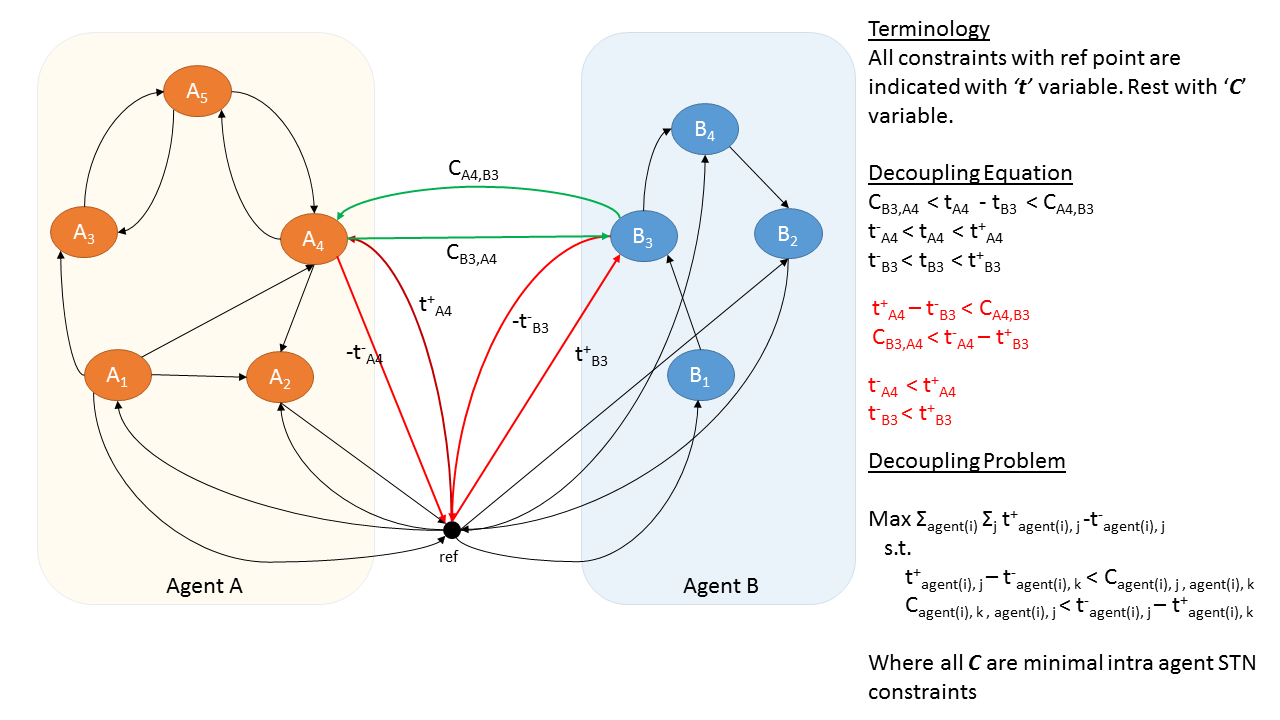
\includegraphics[width = 1.0	\textwidth]{Decoupling_figures.png}
%    \caption{Decoupling }
\end{figure}
\end{frame}

%------------------------------------------------
\section{Problem Formulation}
%------------------------------------------------
\begin{frame}
\frametitle{Problem Formulation}
\FontviTen
The N agent decoupling problem is mathematically represented as follows-:
\begin{align*}
\text{$\mathrm{min}$ } & \text{  $\sum_{i=1}^{N} f_i$} \\
\text{subject to} & \\
&\begin{bmatrix}
B_{1} & B_{2} & B_{3} & . & . & . & B_{N}  \\
A_{1} &  0      &  0  & 0 & 0 & 0 &  0     \\
0     &  A_{2}  &  0  & 0 & 0 & 0 &  0     \\
.     &  .  &  .  & . &. & . &  .     \\
0     &  0      &  0  & 0 & 0 & 0 &  A_{N}  
\end{bmatrix}
\begin{bmatrix}
X_1 \\ X_2 \\ . \\ . \\ X_{N}
\end{bmatrix}
\leq
\begin{bmatrix}
b \\ c_1 \\ c_2 \\ . \\ c_N
\end{bmatrix}
\end{align*}
\begin{eqnarray}
M_i &\rightarrow& \text{ Number of time point variables in agent i } \nonumber\\
X_i &\in& R^{M_i \choose 2} \times 1 \nonumber \\
\sum_{i=1}^{N} B_i X_i &\leq& b \rightarrow \text{Inter-agent coupling constraints} \nonumber\\
A_i X_i &\leq& c_i , i = 1..N \rightarrow \text{Intra-agent triangular consistency constraints} \nonumber \\ 
rows(A_i)&\rightarrow& {M_i \choose 3} \nonumber
\end{eqnarray}
\end{frame}
%------------------------------------------------
\section{Assumptions}
%------------------------------------------------
\begin{frame}
\frametitle{Assumptions}
\begin{itemize}
\item The objective function $f_i$ is private to agent $i$.
\item The number of colluding agents is known to all agents.
\item Agent \textit{i} is aware of matrices $A_i$ and $c_i$.
\item Agent \textit{i} is only aware of the constraints that it participates in the equation $\sum_{i=1}^{N} B_i X_i \leq b$. 
\begin{enumerate}
\item Agent \textit{i} is aware of matrix $B_i$.
\item \textcolor{red}{Suppose agents \textit{i} and \textit{j} share a coupling constraint between time point variables $t_{m,i}$ and $t_{n,j}$, then agent $i$ has access to $t_{n,j}^{+}$ and $t_{n,j}^{-}$. Similarly  agent $j$ has access to $t_{m,i}^{+}$ and $t_{m,i}^{-}$.}
\end{enumerate}
\item Two agents are allowed to communicate directly with each other only if there exists a coupling constraint between them.
\end{itemize}
\end{frame}

%------------------------------------------------
\section{Optimization Algorithm}
%------------------------------------------------
\subsection{Lagrange Dual Basics}
\begin{frame}
\frametitle{Lagrangian Dual Basics}
\FontviNine
Consider the primal and its Lagrangian dual. If functions $f(x), g(x)$ and set $\Omega$ are convex, $h(x)$ is affine, then primal and dual optimum are equal.

\begin{columns}[t] % The "c" option specifies centered vertical alignment while the "t" option is used for top vertical alignment

\column{.2 \textwidth} % Left column and width
\begin{align*}
&\textbf{Primal Problem}\\
& \mathrm{ min } \,\, f(x)\\
\text{sub} & \text{ to} \\
& g(x) \leq 0 \\
& h(x) = 0 \\
& x \in \Omega 
\end{align*}

\column{.2\textwidth} % Right column and width
\begin{align*}
&\textbf{Lagrangian Dual Problem}\\
&\underset{\lambda \geq 0 , \nu}{\mathrm{max}}\,L(\lambda,\nu) = \underset{x}{\mathrm{inf}} \,\, f(x) + {\lambda }^{T} g(x) + {\nu}^{T} h(x)\\
\text{sub} & \text{ to}\\
& x \in \Omega 
\end{align*}
\end{columns}
Using the above duality relationship, our problem can be formulated as 
\begin{align*}
&\underset{\nu}{\mathrm{max}}-{\nu}^{T}b + \sum_{i=1}^{N} \underbrace{\textcolor{red}{ \underset{X_i}{\mathrm{inf}} \,\,f_{i}(X_i) + {\nu}^{T} B_i X_i}}_{L_{i}(v)}  \\
\text{sub} & \text{ to} \\
&A_i X_i = c_i , i = 1,..,N 
\end{align*}
The above problem reduces to an unconstrained optimization problem w.r.t $\nu$.
\end{frame}

%------------------------------------------------
\begin{frame}
\frametitle{Lagrange Dual Basics Contd...}
\FontviNine
The dual objective $L(\nu)$ is a concave function. Algorithm \ref{Sub-gradient} is a simple ascent algorithm maximizing $L(\nu)$ using steepest gradient.
\begin{algorithm}[H]
\caption{Sub-Gradient Algorithm }
\label{Sub-gradient}
\textbf{Parameters:} $\nu^0$
\begin{algorithmic}[1]
\Procedure{Sub-gradient Ascent}{}
\For{k $\geq$ 0} 
\State $X_i^{*} = \mathrm{arg min} \left\lbrace f_i(X_i) + \nu^k B_i X_i\right\rbrace$ sub to. $A_i X_i = c_i , \,\forall i= 1 .. N$
\State $\Delta \nu = \left( \sum_{i = 1}^{N} B_i X_i^{*} \right) - b$ , \text{$\Delta \nu\,$ is a sub-gradient}
\State $\nu^{k+1} = \nu^k + c_k \Delta \nu$, \text{Step-size $c_k$ is computed via line search}  
\State k = k + 1
\EndFor
\EndProcedure
\end{algorithmic}
\end{algorithm}
\textcolor{red}{If f(x) is not strictly convex, then L($\nu$) is not differentiable. Convergence is sub linear.}
\end{frame}

%------------------------------------------------
\subsection{Self Concordance}
%------------------------------------------------
\begin{frame}
\frametitle{Self Concordance}
\begin{enumerate}
\item A function $g$ is said to be self concordant if 
\begin{equation}
\lvert g'''(x)\rvert\ \leq 2 \lvert g''(x) \rvert ^{3/2} \nonumber
\end{equation}
\item Strictly convex self concordant (SCSC) functions have positive Hessian, hence 2nd order methods such as Newtons method can be applied.
\item \textcolor{red}{Minimizing a strictly convex self concordant function using Newton's method is polynomial.}
\item IPM's for optimizing linear and quadratic objectives add barrier terms such that the augmented function is self concordant.
\item To exploit self concordance, we will modify the objective by augmenting a self concordant barrier i.e. $f(x) + t \phi(x)$.
\item Newton's decrement $\lambda(x) = -((\Delta x_{nt})^T \nabla^2 g^{-1}(x) (\Delta x_{nt}) )$ is an provable estimate of $g(x) - p^{*} < (0.68)^2$ when $\lambda(x) \leq 0.68 $.
\end{enumerate}
\end{frame}
%------------------------------------------------
\subsection{Problem Reformulation}
%------------------------------------------------
\begin{frame}
\frametitle{Problem Reformulation}
\FontviTen
The decoupling problem is reformulated as follows-:
\begin{align*}
R(t) = &\underset{\nu}{\mathrm{max}}-{\nu}^{T}b + \textcolor{red}{\sum_{i=1}^{N} \underbrace{\underset{X_i}{\mathrm{inf}} \,\,f_{i}(X_i) + t\phi_i(X_i) + {\nu}^{T} B_i X_i}_{L_{i}(\nu,t)}} , t > 0  \\
\text{sub} & \text{ to} \\
&A_i X_i = c_i , i = 1,..,N 
\end{align*}
\begin{itemize}
\item $f_{i}(X_i) + t\phi_i(X_i) + {\nu}^{T} B_i X_i$ is self concordant by construction. However we require $L_i(\nu,t)$ to be self concordant w.r.t $\nu$. 
\item Turns out that $L_i(\nu,t)$ is related to Legendre transformation of $-f_{i}(X_i) - t\phi_i(X_i)$ via affine transformation.
\item \textcolor{blue}{Since by construction $f_{i}(X_i) + t\phi_i(X_i)$ is self concordant, $L_i(\nu,t)$ has negative definite Hessian (w.r.t $\nu$) and is bounded on $X_i$. Hence $L_i(\nu , t)$ is also self concordant.}  
\item \textcolor{violet}{The optimal value to our problem is $\underset{t \rightarrow 0}{lim} R(t)$.}
\end{itemize}
\end{frame}

%------------------------------------------------
\begin{frame}
\frametitle{ How to Obtain self concordant $\phi(x)$ ? }
\FontviTen 
\begin{itemize}
\item $\forall y_j \in X_i$, we bound $l_j \leq y_j \leq u_j$. Then $\phi_i(x) = -\sum_{y_j \in X_i} log(u_j - y_j)log(y_j - l_j)$. 
\item We exploit the property that edge weights (treated as variables) in a STN can only reduce by adding constraints.
\item Initially each agent omits coupling constraints and computes a minimal STN.
\item Let $u_j$ be the value of $y_j$ in the minimal STN of Agent $i$, say. Then $y_j \leq u_j$ with coupling constraints considered.
\item To compute $l_j$, we consider the set ($\omega_j$) of all closed paths of length 2 and 3 involving $y_j$ in the minimal STN. All such path costs must be $\geq$ 0. 
\item Let the $m^{th}$ element of $\omega_j$ be $\left[c_{1} , c_{2} , y_j\right]$. Then 
\begin{eqnarray}
\label{triangleconstraint}
\label{const1}
&d_m = c_1 + c_2 \\
\label{const2}
&y_j \geq -d_m \\
&\ref{const1} \text{ \& } \ref{const2} \implies y_j \geq \mathrm{max} \left\lbrace -d_m \right\rbrace \forall m \nonumber
\end{eqnarray}
\end{itemize}
\end{frame}

%------------------------------------------------
\subsection{Optimization Algorithm}
\begin{frame}
\frametitle{Optimization Algorithm \cite{p1}}
\FontviNine
We use Newton's method for optimizing $L_i(\nu,t)$ w.r.t $\nu$. The Newton's step is given by
\begin{eqnarray}
\Delta \nu &=& \left(\nabla_{\nu}^2 L(\nu,t)\right)^{-1} \nabla_{\nu}L(\nu,t) \nonumber\\
\nabla_{\nu}L(\nu,t) &=& b + \sum_{i=1}^{N} \nabla_{\nu}L_{i}(\nu,t) \nonumber \\
&=& \textcolor{red}{b-\sum_{i=1}^{N} B_i X_i(\nu,t)} \text{ , where }\nonumber\\
X_{i}(\nu,t) &=& \mathrm{arg\,min}\, f_{i}(X_i) + t\phi_i(X_i) + {\nu}^{T} B_i X_i \text{ s.t } A_i X_i = c_i \nonumber\\
\left(\nabla_{\nu}^2 L(\nu,t)\right) &=& \sum_{i=1}^{N}\textcolor{red}{\left(\nabla_{\nu}^2 L_{i}(\nu,t)\right)} \nonumber\\
\text{Let }H_i(\nu,t) &=& \nabla_{\nu}^2 f_i(X_i(\nu,t)) + t \nabla_{\nu}^2 \phi_i(X_i(\nu,t)) , \text{ then} \nonumber
\end{eqnarray}
\begin{equation}
\left(\nabla_{\nu}^2 L_{i}(\nu,t)\right) = B_i\left[{H_{i}(\nu,t)}^{-1} - {H_i(\nu,t)}^{-1}{A_i}^T \left(A_i {H_i(\nu,t)}^{-1} {A_i}^{T} \right)^{-1} A_i {H_{i}(\nu,t)}^{-1} \right] {B_{i}}^{T} \nonumber
\end{equation}

\end{frame}

%------------------------------------------------
\begin{frame}
\frametitle{Optimization Algorithm Contd...}
\FontviNine
Initialization of the path following algorithm,
\begin{algorithm}[H]
\scriptsize
\caption{Initialization Of Path}
\textbf{Input:} $\nu^0 , t^0 , \epsilon > 0 , k = 0$
\begin{algorithmic}[2]
\Procedure{Path Initialization}{}
\While{(1)} 
\State Compute $X_i(\nu^k , t^0)\forall i$. $\delta_k = \delta(\nu^k , t^0)$
\Comment{\textcolor{red}{$X_i$ are computed separately by each agent subject to $A_i X_i = c_i$}}
\If{$\delta_k \leq \epsilon$}
\State return $\nu^k $ 
\EndIf
\State $\nu^{k+1} = \nu^k + \sigma \Delta\nu(\nu^k , t_0)$ 
\Comment{$\sigma$ is a suitable step length}
\State k = k + 1
\EndWhile
\EndProcedure
\end{algorithmic}
\end{algorithm}
Newton's Decrement- $\delta(\nu^k , t^0) = \textcolor{blue}{\frac{\alpha}{2}} \sqrt{\nabla_{\nu}L(\nu^k,t)^{T} \left(\nabla_{\nu}^2 L(\nu^k,t)\right)^{-1} \nabla_{\nu}L(\nu^k,t)}$
\textcolor{red}{Computation of $\delta(\nu^k , t^0)$ is through a distributed summation.}
\end{frame}
%------------------------------------------------
\begin{frame}
\frametitle{Optimization Algorithm Contd...}
\FontviNine
\textcolor{red}{Path following algorithm initialized with previously found $\nu$.}
\begin{algorithm}[H]
\scriptsize
\caption{Path Following}
\textbf{Input:} $\nu^0 , t^0 , \epsilon > 0$ satisfying $\delta{(\nu^0 , t^0)} \leq \epsilon, 0 < \tau < 1$
\begin{algorithmic}[3]
\Procedure{Path Following}{}
\While{(1)} 
\If{$t^k N_{\phi} \leq \epsilon$}
\State{break}
\EndIf
\State $t^{k+1} = \tau t^{k}$
\State Initialize $\nu = \nu^{k} , t = t^{k+1} , \delta = \delta(t^{k+1} , \nu^{k})$
\While{$\delta \geq \epsilon$}
\State Compute $X_i = X_{i}(\nu, t) \forall i$.
\Comment{\textcolor{red}{$X_i$ computed separately by each agent subject to $A_i X_i = c_i$}}
\State $\nu^{+} = \nu + \sigma \Delta(\nu , t)$
\Comment{\textcolor{red}{$\sigma$ is a suitable step length}}
\State $\delta^{+}= \delta(\nu^{+},t)$ , Update $\nu = \nu^{+} , \delta = \delta^{+}$
\Comment{\textcolor{red}{$\delta^{+}$ computed via distributed summation}}
\EndWhile
\State $\nu^{k+1} = \nu$ and $X_{i}^{k+1} = X_i \, \forall i$
\Comment{\textcolor{red}{$X_{i}^{k+1}$ is feasible to all agents respecting coupling constraints}}
\EndWhile
\EndProcedure
\end{algorithmic}
\end{algorithm}
\end{frame}
%------------------------------------------------
\section{Network Communication}
\begin{frame}
\frametitle{Network Communication}
\FontviTen
\begin{itemize}
\item Recall that communication over the N/W is required for computation of $\delta$.
\item Specifically $\nabla_{\nu}L(\nu,t)$ and $\nabla_{\nu}^2 L(\nu,t)$ needs to be computed distributively. Computation of $\sigma$ ??
\item Depending on the project requirements, different network topologies can be devised. 
\item For minimizing N/W communication a minimum spanning tree can be constructed in a distributed fashion.
\item This N/W topology allows only agents sharing a coupling constraint to communicate with each other.
\end{itemize}
\begin{figure}
\centering
    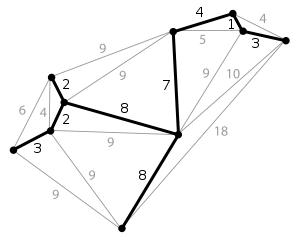
\includegraphics[width = 0.3\textwidth]{Minimum_spanning_tree.png}
    \caption{Spanning tree. Image taken from \cite{p2}}
\end{figure}
\end{frame}
%------------------------------------------------
%----------------------------------------------------------------------------------------
\section{Some Thoughts About The Method}
\begin{frame}
\frametitle{Some Thoughts About The Method}
\FontviNine
\begin{block}{Agent Coordination}
Agents must coordinate in some fashion for creation of coupling matrix $B$. Specifically, each agent must assume responsibility for a specific row in $B$.
\end{block}

\begin{block}{Feasible Solutions}
After every outer iteration we get a feasible solution to our original problem. 
\end{block}

\begin{block}{Infeasibility Check}
If the problem is infeasible, then the function $L(\nu,t)$ will assume the value $\infty$.
\end{block}

\begin{block}{Number of Outer Iterations}
The number of outer iterations is given by $log_{\tau}{\frac{\epsilon}{N_{\phi} t_0}}$, $\epsilon \rightarrow$ level of accuracy. \textcolor{red}{$N_{\phi} = \sum_{i=1}^{N} N_i$}, $N_i \rightarrow$ no. of time point variables in agent i.
\end{block}
\end{frame}

\begin{frame}
\frametitle{Some Thoughts About The Method Contd...}
\FontviNine
\begin{block}{Choosing $\sigma$ for line search}
\textcolor{red}{Usually line search techniques which satisfy Armijo's criteria are used and in the process will reveal private objective values of the agents. If agents do not want to share those values, we can use a prescribed step length using $\delta$.}
\end{block}

\begin{block}{Distributed Computation}
During distributed summation of $\nabla_{\nu} L(\nu , t)$ there is a chance that some values of time points may be revealed to a non associated agent. To avoid this we multiply each row in matrix $B$ by a random number that is known only to the agents concerned.
\end{block}

\begin{block}{Complexity}
Polynomial!
\end{block}
\end{frame}

%%------------------------------------------------
\begin{frame}
\frametitle{References}
\footnotesize{
\begin{thebibliography}{99} % Beamer does not support BibTeX so references must be inserted manually as below
\bibitem[Necoara et.al, 2009]{p1} Necoara, I and Suykens, JAK (2009)
\newblock Interior-point lagrangian decomposition method for separable convex optimization
\newblock \emph{Journal of Optimization Theory and Applications} Springer pp 567--588 
%------------------------------------------------
\bibitem[Wikipedia]{p2} Minimum Spanning trees
\newblock \emph{https://en.wikipedia.org/wiki/Minimum\_spanning\_tree} 12(3), 45 -- 678.
\end{thebibliography}
}
\end{frame}

%\section{Second Section}
%%------------------------------------------------
%
%\begin{frame}
%\frametitle{Table}
%\begin{table}
%\begin{tabular}{l l l}
%\toprule
%\textbf{Treatments} & \textbf{Response 1} & \textbf{Response 2}\\
%\midrule
%Treatment 1 & 0.0003262 & 0.562 \\
%Treatment 2 & 0.0015681 & 0.910 \\
%Treatment 3 & 0.0009271 & 0.296 \\
%\bottomrule
%\end{tabular}
%\caption{Table caption}
%\end{table}
%\end{frame}

%------------------------------------------------
\bibliography{Master}
\end{document} 